\documentclass[12pt]{article}
\usepackage[spanish,es-tabla]{babel}
\usepackage{graphicx}
\usepackage{wrapfig}
\usepackage[a4paper]{geometry}
\usepackage{amsmath}
\usepackage{mathtools}
\usepackage{multicol}


\geometry{top=1.5cm, bottom=1.5cm, left=1.25cm, right=1.25cm}
\newcommand*{\grabto}[2]{\IfFileExists{#2}{}{\immediate\write18{curl \detokenize{#1 -o #2}}}}

%\grabto{https://i.ibb.co/c1ChB49/photo-2022-10-15-17-12-01.jpg}{esquema.png}
%\grabto{https://i.ibb.co/c1ChB49/photo-2022-10-15-17-12-01.jpg}{esquema_momentos.png}


\begin{document}
    
        \begin{center}
            \section{Diseño de Placa Base}
        \end{center}

        \subsection{Propiedades de los Materiales}

        \begin{wrapfigure}{r}{0.25\textwidth}
            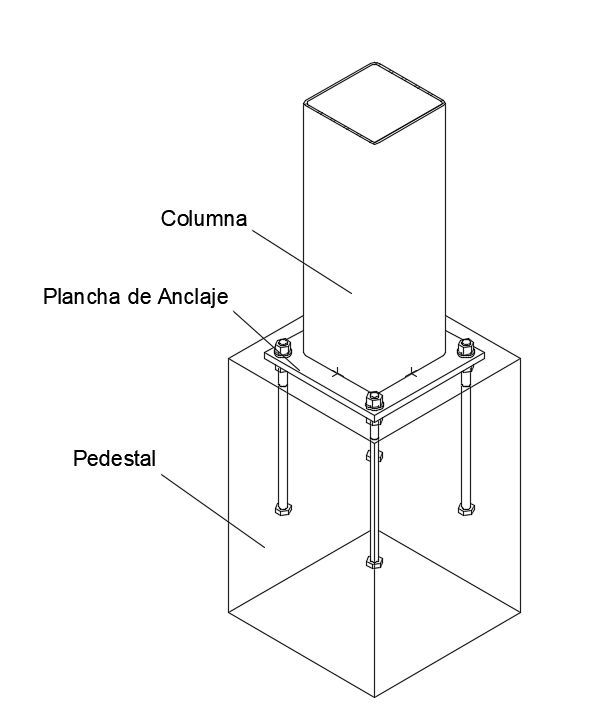
\includegraphics[width=0.25\textwidth]{esquema.png}
        \end{wrapfigure}

        \noindent \textbf{Acero}

        \begin{tabular}{l l}
            Tensión cedente de la columna:& $F_{yc} = 250 MPa$ \hspace{20cm}\\
            Factor de sobreresistencia:& $R_{y}=1.5$ \\
            Tensión cedente de la placa base:& $F_{ypl} = 250 MPa$ \\
            Tensión última en la placa base:& $F_{upl} = 400 MPa$ \\
            Módulo de elasticidad:& $E = 200 000 Mpa $ \\ \\
        \end{tabular}  


        \noindent \textbf{Concreto:}\\ 
        \indent Resistencia a la Compresión del concreto: $f'_{c} = 210 kgf/cm^{2} $
    
        \subsection{Cargas de diseño}
        \begin{tabular}{llll}
            Combo 1 & $P_{u}=14357.14 kgf$ & $M_{ux} = 5787.32 kgf \cdot cm $ & $M_{uy} = 5787.32 kgf \cdot cm $ \\
        \end{tabular}
     
        \subsection{Dimensiones de columna}
        \begin{tabular}{ll}
            Ancho de la sección:& $b = 15 cm$ \hspace{15cm} \\
            Alto de la sección:& $a = 15 cm$ \\
            Módulo plástico:& $Z_{xc} = 2683 cm^3 $ \\
            Altura de piso:& $h=2.70m$
        \end{tabular}
    
        \subsection{Factores de resistencia}
        \noindent$\phi_{c} = 0.65$ (Resistencia al corte) \\
        $\phi_{f} = 0.90$ (Resistencia a la compresion)\\
        
        \subsection{Dimensiones de pedestal}
        $a = 40 cm \qquad b = 40 cm \qquad A_{ped} = a \cdot b = 1600 cm^{2} $   \\

        \subsection{Resistencia Requerida}
        \noindent Momento máximo incluyendo sobreresistencua y endurecimiento del acero: \\
        $M_{u} = 1.1 \cdot R_y \cdot F_{yc} \cdot Z_{xc} = 1106 kN \cdot m $ \\
        Resistencia requerida por corte (en función al momento máximo probable de la columna)\\
        $M_{pc} = R_{y} \cdot F_{yc} \cdot Z_{xc} = 10006.13 kN \cdot m $ \\
        $ V_{u} = \frac{2 \cdot M_{pc}}{H} = 628.83 kN \hspace{15cm} $

    \section{Comprobación de las barras de anclaje}
    \begin{minipage}{\textwidth}

        \begin{wrapfigure}{rh}{0.4\textwidth}
            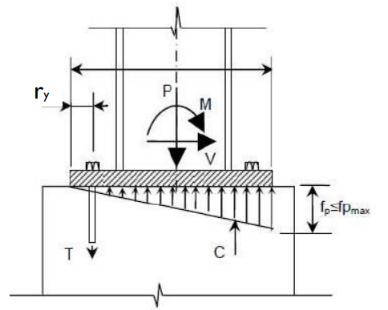
\includegraphics[width=0.4\textwidth]{esquema_momentos.png}
        \end{wrapfigure}
        
        \begin{align*}
            &\text{Excentricidad equivalente debido a la flexión:} \\
            &e = \frac{M_u}{P_u} = 388 mm \\
            &\text{Factor de minoración de resistencia del concreto:} \\
            &\phi_{c} = 0.65\\
            &\text{Esfuerzo máximo entre la placa base y el concreto:} \\
            &f_{pmax} = \phi_c \cdot 0.85 \cdot f'_c \sqrt{\frac{A_{pedestal}}{A_{placa}}} = 18.27 MPa \\
            &\text{Fuerza máxima entre la placa base y el concreto (unitario):}\\
            &q_{\max} = f_{pmax} \cdot B = 91.36 kN/cm\\
            &\text{excentricidad críticas:}\\
            &e_{crit} = \frac{N}{2}-\frac{P_y}{2 \cdot q_{\max}} = 207.36 cm \\
            &\text{Verificación por Momentos Altos:}\\
            &e>e_{crit} \text{\ldots Momentos Altos}\\
            &\text{Separación entre la barra al borde de la placa} (\min 1.5\cdot d_r)\\
            &r_y = 50 mm \\
            &\text{Distancia del centro de la placa base a la fila de barras más traccionada:}\\
            &f = 230 cm \\
        \end{align*}
    \end{minipage}

    \noindent \textbf{Momentos bajos:} \\
    Las fuerzas de tensión son resistidas íntegramente por el concreto, no es necesaria una comprobación de las barras por tracción.\\ \\
    Ancho en compresión para momentos bajos:\\
    $Y_{mb} = N-2e=-216.17 mm$ \\ \\
    Fuerza entre la placa base y el concreto
    \begin{align*}
        &q = \frac{P_u}{Y} = 9136.11 kN/m \hspace{15cm}\\
        &f_p = \frac{q}{B} = 18.27 MPa
    \end{align*}


    \noindent Revisión por aplastamiento en el pedestal \\
    $f_{pmax} > f_{p} \cdots OK$ \\

    \noindent \textbf{Momentos Altos:} \\
    Comprobando si el área resistente es mayor al área requerida:
    \begin{align*}
        &A_{res} = {\left( f+\frac{N}{2} \right) }^2=2601 cm^2 \hspace{15cm}\\
        &A_{req} =\frac{2P_u \cdot (e+f) }{q_{\max}} = 1796 cm^2 \\
        &A_{res} > A_{req} \cdots OK
    \end{align*}

    \noindent Cálculo del ancho en compresión para momentos altos:
        \begin{align*}
            &Y_{ma1} = \left( f+\frac{N}{2} \right) + \sqrt{{\left( f+\frac{N}{2} \right)}^2 -\frac{2 Pu_u \cdot (e+f) }{q_{\max}}} \hspace{15cm} \\
            &Y_{ma1} = \left( f+\frac{N}{2} \right) - \sqrt{{\left( f+\frac{N}{2} \right)}^2 -\frac{2 Pu_u \cdot (e+f) }{q_{\max}}} \\
            &Y_{ma} = 226.27 mm 
        \end{align*}
    
    \noindent \textbf{Resistencia del Anclaje a la tracción}
        \begin{align*}
            &\text{Fuerza entre la placa base y el concreto} \hspace{15cm} \\
            &q = q_{\max} = 9136.11 kN/m \\
            &\text{Fuerza última en las barras de tracción} \\
            &N_{uag}=q \cdot Y - P_u = 739.87 kN \\
            &\text{Fuerza crítica en las barras de anclaje (número de barras resistenentes = $n_r$ = 4)}  \\
            &N_{ua} = \frac{N_{uag}}{n_r} = 184.97 kN\\
            &\text{Tensión última a tracción de la barra de anclaje:} \\
            &F_{barra} = 861.81 MPa \\
            &\text{Factor de minoración}\\
            &\phi = 0.75 \\
            &\text{Área efectiva de la barra de anclaje}\\
            &A_{barra} = \frac{\pi}{4} {(d_r)}^ 2 = 3.18 cm^2 \\
            &\text{Resistencia Minorada a tracción de la barra de anclaje:}\\
            &N_{barra} = \phi \cdot F_{barra} \cdot A_{barra} = 205.38 kN\\
            &\text{Relación resistencia / Fuerza aplicada a las barras:} \\
            &Ratio = \frac{N_{barra}}{N_{ua}} = 0.901 < 1 \cdots OK
        \end{align*}  
        
        \subsection{Espesor de la Plancha} 
            \begin{align*}
                &m = 0.5 \cdot (N-0.95 \cdot d) = 5.375 cm \text{\hspace{15cm} } \\
                &n = 0.5 \cdot (B-0.80 \cdot b) = 6.5 cm \\
                &X = \left( \frac{4 \cdot A_{\min} }{{(b+d)}^{2}} \right) \cdot \frac{P_u}{\phi P_p} = 0.198 \\
                &\lambda = \min \begin{cases} \frac{2 \cdot \sqrt{X} } {1+\sqrt{1-X} } \\ 1 \end{cases}  = 0.469 \\
                &n' = \frac{\sqrt{A_{\min}}}{4} =  3.75 cm \\
                &l = \max \begin{cases} m \\ n \\ \lambda \cdot n' \end{cases}  = 6.5 cm \\
                &t = \sqrt{\frac{2 \cdot P_u \cdot l^2 } {0.90 \cdot F_y \cdot A_1 }} = 0.923 cm
            \end{align*}

        \textbf{Dimensiones de la plancha de anclaje}\\
        $B=0.25 m \qquad N=0.25 m \qquad t = 1.5 cm$
        

    \section{Revisión a Corte:}
        \begin{align*}
            &V_u = \sqrt{{66.81kgf}^2+{44.84kgf}^2} = 82.758 kgf \hspace{15cm}  \\
            &n_{corte} = 4 \\
            &F_{barras} = 0.5*36 ksi = 124.106 MPa \\
            &\phi = 0.75 \\
            &d_p = \frac{5}{8} in \\
            &\phi P_{barras} = \phi \cdot F_{barras} \cdot A_r = 1878.665 kgf \\
            &Ratio = \frac{V_u}{\phi \cdot P_{barras} \cdot n_{corte} } = 0.11
        \end{align*}
\end{document}